
\documentclass[a4paper,11pt,fleqn]{article}
\usepackage{amsfonts}
\usepackage{amsthm}
\usepackage{graphicx}

\setlength{\parindent}{3em}
\setlength{\oddsidemargin}{0in}
\setlength{\textwidth}{6.5in} % sets 1in left and right margins
\setlength{\topmargin}{0.0in} % change to 0.2in for regular latex
%\setlength{\headheight}{0in}
%\setlength{\footheight}{0.5in}
\setlength{\footskip}{0.5in}
\setlength{\textheight}{9.0in} %sets 1in top and bottom margins
%\renewcommand{\baselinestretch}{1} %set to 1.5 for double spacing.


\newtheorem{Prop}{Proposition}
\newtheorem{lemma}{Lemma}

\newcommand{\br}{{\mathbf r}}
\newcommand{\bA}{{\mathbf A}}
\newcommand{\ba}{{\bf a}}
\newcommand{\bb}{{\bf b}}
\newcommand{\bc}{{\bf c}}
\newcommand{\bC}{{\bf C}}
\newcommand{\bd}{{\bf d}}
\newcommand{\be}{{\bf e}}
\newcommand{\bs}{{\bf s}}
\newcommand{\bn}{{\bf n}}
\newcommand{\bu}{{\bf u}}
\newcommand{\bv}{{\bf v}}
\newcommand{\bw}{{\bf w}}
\newcommand{\bx}{{\bf x}}
\newcommand{\by}{{\bf y}}
\newcommand{\bbf}{{\bf f}}
\newcommand{\bE}{{\bf E}}
\newcommand{\bL}{{\bf L}}
\newcommand{\bM}{{\bf M}}
\newcommand{\bN}{{\bf N}}
\newcommand{\bS}{{\bf S}}
\newcommand{\bT}{{\bf T}}
\newcommand{\bD}{{\bf D}}
\newcommand{\bX}{{\bf X}}
\newcommand{\bP}{{\bf P}}
\newcommand{\bI}{{\bf I}}
\newcommand{\bR}{{\bf R}}
\newcommand{\bU}{{\bf U}}
\newcommand{\bV}{{\bf V}}
\newcommand{\bW}{{\bf W}}
\newcommand{\bJ}{{\bf J}}
\newcommand{\bB}{{\bf B}}
\newcommand{\bzero}{{\bf 0}}
\newcommand{\bgamma}{{\mbox {\boldmath $\gamma$}}}
\newcommand{\btheta}{{\mbox {\boldmath $\theta$}}}
\newcommand{\bLambda}{{\mbox {\boldmath $\Lambda$}}}
\newcommand{\bPsi}{{\mbox {\boldmath $\Psi$}}}
\newcommand{\bPhi}{{\mbox {\boldmath $\Phi$}}}
\newcommand{\bcS}{{\mbox {\boldmath ${\cal S}$}}}
\newcommand{\bcH}{{\mbox {\boldmath ${\cal H}$}}}
\newcommand{\bcI}{{\mbox {\boldmath ${\cal I}$}}}
\newcommand{\bcR}{{\mbox {\boldmath ${\cal R}$}}}
\newcommand{\bcB}{{\mbox {\boldmath ${\cal B}$}}}

\title{One-Shot Semi-Blind Decorrelating Detection Algorithms with Multiple Windows for Asynchronized CDMA}
\date{}
\author{Shu Wang, James Caffery and Hanhong Shen}
\begin{document}
\maketitle

\begin{abstract}
Multiuser detection is one of the key techniques for combating
multiple access interference (MAI) in CDMA systems. In this paper,
we propose two effective direct multiuser semi-blind decorrelating
multiuser detectors with multiple windows, which only require the
perfect timing, the amplitude/power and signature of the signal
sent by the desired user. Both of these two semi-blind detectors
are based on the classic truncated-window decorrelating detector.
But a new semi-blind signature matrix is employed. Furthermore, in
order to compensate the performance degrading of the classic
truncated-window decorrelating detector, a new
multi-truncated-windows scheme is proposed to detect several
consecutive bits sent by the desired user at the same time. So,
these detectors could achieve least squares, near-far resistance
and maximum-likelihood and achieve the same optimum performance of
the classic truncated-windows decorrelating detector in some
situations. These two algorithms are simple and direct, They don't
require any knowledge of the other users. There is also no any
search or adaptive procedure in these two algorithm. Theoretical
analysis and computer simulations are also presented to support
the performance of the present algorithms.
\end{abstract}

\section{Introduction}

Direct-sequence code division multiple access (DS/CDMA) techniques
have attracted increasing attention for efficient use of available
bandwidth, resistance to interference and flexibility to variable
traffic patterns. One of the problems of such a system is the
so-called near-far problem resulting from excessive multiple
access interference (MAI) energy from nearby users compared with
the desired user's signal energy. Multiuser detection strategy is
a method to minimize the effect of MAI and solve the near-far
problem in CDMA systems without a significant reduction in the
signal energies of the strong users in order for the weaker users
to achieve reliable communication . It has been extensively
investigated over the past several years ~\cite{Verd98}, since MAI
is the dominant impairment for CDMA systems and exists even in
perfect power-controlled CDMA systems. Most early work on
multiuser detection assumed that the receiver knew the spreading
codes or had some knowledge of all users, then exploited this
knowledge to combat MAI. For example, the classic decorrelating
detector for the synchronous case or the truncated-window
decorrelating detector could achieve the optimum near-far
resistance and completely eliminate MAI from other users with the
expense of enhancement of background noise. However, in many
practical cases, especially in a dynamic environment, e.g. in the
downlink of the CDMA system, it is very difficult for a mobile
user to obtain accurate information on other active users in the
same channel. On the other hand, the frequent use of training
sequence is certainly a waste of channel bandwidth. So blind
multiuser detection has been proposed. Recent research has been
devoted to the multiuser blind receivers and subspace-based
signature waveform estimation schemes to achieve better
performance and higher capacity~\cite{Honi95, Poor97, Wang98,
Torl97, Liu96}. The Minimum output energy (MOE) method and
subspace method were presented for multiuser blind detection with
the knowledge of only the desired users' spreading code and
possible timing.

An optimum near-far resistant multiuser detector which dose not
need power control has been proposed by Verd\'u ~\cite{Verd89}.
However, its complexity is exponential in terms of he number of
users, which makes it unsuitable for practical situations. The
large gaps in performance and complexity between the conventional
single-user matched filter and optimum multiuser detector
encourage the search for other multiuser detectors that exhibit
good performance/complexity tradeoffs. Suboptimum linear
detectors, which are based on linear transformation of the sampled
match filter outputs, were considered in ~\cite{Lupa89} for
synchronous case. The decorrelating detector ~\cite{Lupa89} not
only is a simple and nature strategy but it is optimal according
to three different criteria: least squares, near-far resistance
~\cite{Verd86} and maximum-likelihood when the received amplitudes
are unknown ~\cite{Lupa89}. Though it does not require knowledge
of the received amplitudes, it does require the information about
other active users' signature waveforms. For the asynchronous
cases, Verd\'u suggested to use a one-shot version of his
decorrelating detector, the truncated-window decorrelating
detector, in which $1+2(K-1)=2K-1$ filters, where $K$ is the
number of users, are matched to one full code of a specific user
(without loss of generality, called the first user) and two
filters matched to each of the other users. One filter is matched
to the \textquotedblleft previous\textquotedblright\ part of its
code, corresponding to the time between zero and $\tau_k$, where
$\tau_k$ is the delay of user $k$ with respect to the first user,
and to the \textquotedblleft current\textquotedblright\ part of
the code, corresponding to the time between $\tau_k$ and $T$. In
this case, it not only requires the information about other active
users' signatures but also the time delay of other users with
respect to the first user. However, since only the signature
information of the other users is divided in a signature matrix of
the nearly doubled size, the performance of this one-short
decorrelating detector is worse than the complete asynchronouse
decorrelating detector.

Multiuser blind detection using subspace techniques was first
developed in depth by Wang and Poor ~\cite{Wang98, Poor98}. Such
techniques were appropriate for the downlink environment where
only the desired users' code is available. More recently, these
subspace techniques were extended by Wang and Host-Madsen
~\cite{Wang99}, named group multiuser blind detectors, to uplink
environments where the base station knows the codes of in-cell
users, but not those of users outside the cell. In the
subspace-based blind detection approach ~\cite{Wang98}, the linear
detectors are constructed in the closed form once the signal
subspace components are computed and offer lower computational
complexity and better performance than the blind MOE detector. For
the subspace-based blind adaptive detector, the project
approximation subspace tracking deflation (PASTd) algorithm
~\cite{Yang95} is used to estimate the signal subspace.

It is shown in ~\cite{Honi95} that MOE receiver is equivalent to
the linear minimum mean square error (MMSE) detector, which is
near-far resistant and has much less complexity compared the
optimal multiuser detection. The major limitation of MOE schemes
to multiuser blind detection is that there is a satuaration effect
in the steady state, which causes a significant performance gap
between the converged blind MOE and the true MMSE detector
~\cite{Honi95}.

As we see, various multiuser detection schemes have been developed
to combat the effects of MAI. These detection techniques either
assume the knowledge of all the users in the system (Conventional)
or assume the knowledge of the user of interest and without
knowldege of the channel input (Blind). Due to the limitation of
the blind algorithms in the presence of a large number of
interferers, there is a significant performance gap between these
two classes detector. In this work, we consider an asynchronous
DS/CDMA system and develop some partial blind detectors, a new
least squares (LS) semi-blind multi-window decorrelating detector
(LS-MW) and a total least squares (TLS) semi-blind multi-window
decorrelating detector (TLS-MW), which is expected to bridge the
performance gap between the blind and the conventional multiuser
detectors. In the present multiuser semi-blind detectors, besides
the current user's signature, both the perfect timing of the
desired user and the amplitude of the signature sent by the this
are required. So, we call them semi-blind detectors. In either of
these two algorithms, firstly a new semi-blind signature matrix is
constructed with the current user's signature and amplitude, and
some previously received signal vectors. Then, the decorrelating
operation based on this new blind signature is proposed.
Furthermore, in order to compensate the performance degrading of
the old single-truncated-window scheme, a new multi-window scheme
is proposed and several consecutive bits sent by desired user
would be detected at the same time. Finally, both LS and TLS
version of this semi-blind multi-window decorrelating detection
scheme would be presented with different assumptions. These two
algorithms are are simple joint/block detection algorithms. It is
different to the classic decorrelating detector because that there
is no any requirement of other's information, except the user of
interest. On the other hand,  it is different to any other blind
detection scheme since there is no any adaptive or search
procedure employed. Theoretical analysis and computer simulations
are also present to demonstrate the performance of these two
semi-blind decorrelating detectors.

The rest of the paper is organized as follows. In Section II, we
summarize the signal model. In Section III, we review the classic
decorrelating detector in multiuser detection. In Section IV, the
idea for the semi-blind decorrelating and joint/block detection
scheme is described. In Section V, the new least squares multiuser
semi-blind decorrelating detection algorithm and the total least
squares algorithm are introduced. Performance analysis and
simulation results are provided in Section VI and VII. Section
VIII concludes this papers.

\section{Data Model and Problem Description}

A single-cell symbol-asynchronous DS-CDMA system over the
nondispersive additive white Gaussian noise (AWGN) channel is
considered. Spreading sequences are assigned to users in the
system. The signature waveform of the $k$th user can be expressed
as

\begin{equation}
\begin{array}{rcl}
s_k(t)&=&\sum\limits_{l=0}^{L-1}c_k^{(l)}\psi(t-lT_c)
\end{array}
\end{equation}

\noindent where $c_k^{(l)}\in \{-1/\sqrt{L},\ 1/\sqrt{L}\}$ is the
$l$th chip of the $k$th user, $L$ is the spreading gain, $T_c$ is
the chip interval and $\psi(t)$ is the chip waveform. We assume
that $\psi(t)$ satisfies the Nyquist criterion for zero inter-chip
interference and $\int\limits_{-\infty}^{+\infty}|\psi(t)|^2dt=1$.

We consider reverse link transmission. The baseband representation
of the received signal due to the $k$th user is given by

\begin{equation}
\begin{array}{rcl}
r_k(t)&=&\sum\limits_{i=-\infty}^{+\infty}A_k b_k^{(i)}
s_k(t-iT_c-\tau_k)
\end{array}
\end{equation}

where $b_k^{(i)}$ is the $i$th bit of the $k$th user. We assume
that the $b_k^{(i)}$ are independent and identically distributed
random variables with $E\{b_k^{(i)}\}=0$ and
$E\{|b_k^{(i)}|^2\}=1$. Also, $\tau_k$ denotes the transmission
delay from the $k$th user to the base station and $A_k$ is the
power of the received signal of the $k$th user. Then the baseband
signal at the input to the receiver at the base station is

\begin{equation}
\begin{array}{rcl}
r(t)&=&\sum\limits_{k=1}^{K}r_k(t)+n(t)
\end{array}
\end{equation}

where $n(t)$ is additive white Gaussian noise with power spectral
density $\sigma_{n}^2$. We assume that there are $K$ simultaneous
users in the system.

The received signal is synchronized for each user, passed through
the corresponding chip matched filter (CMF), and sampled at the
chip rate $1/T_c$. The vector of the output samples of the CMF for
$k$th user in the $n$th symbol interval can be expressed as

\begin{equation}
\begin{array}{rcl}
\br_k^{(n)}&=&\left[
\matrix{r_k(nT+T_c+\tau_k)&r_k(nT+2T_c+\tau_k)&\ldots&r_k(nT+LT_c+\tau_k)}\right]^T
\end{array}
\end{equation}

\noindent where

\begin{equation}
\begin{array}{rcl}
r_k(nT+lT_c+\tau_k)&=&\int\limits_{nT+lT_c+\tau_k}^{nT+(l+1)T_c+\tau_k}r_k(t)\psi(t)dt
\end{array}
\end{equation}

\noindent for $1\leq l \leq L$. To facilitate the analysis, we
will assume the system to be chip-synchronous and restrict
ourselves to the receiver that has an observation window of one
symbol interval. Without loss of generality. we consider the
detection of the first user. The observation window of the first
user is marked with a thick line in figure \ref{channel}. The
signals of other users are treated as interference. A typical
interferer has two different but consecutive symbols interfering
the symbol of user $1$, as shown in figure \ref{channel}.

\begin{figure}
\center{
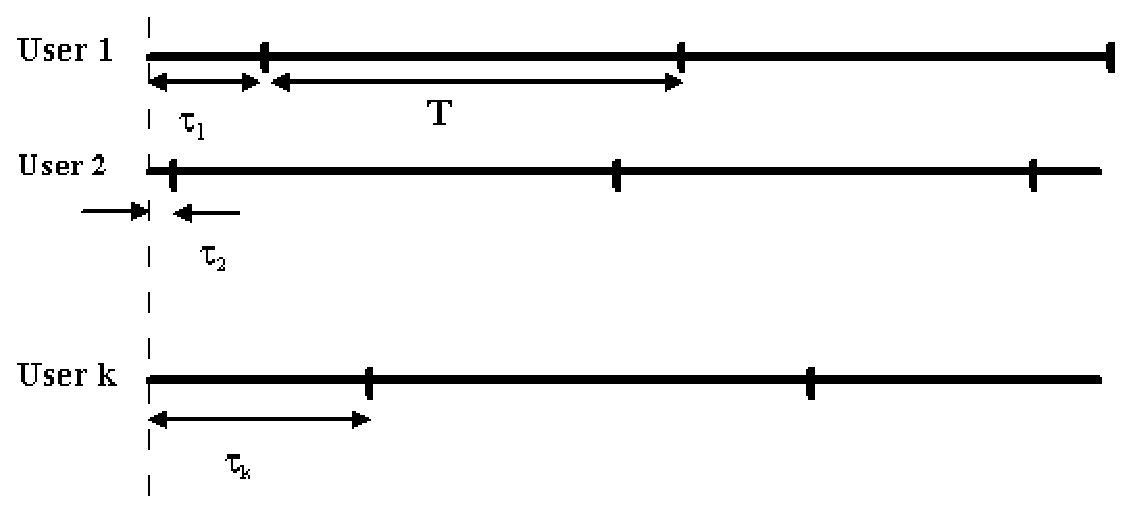
\includegraphics[width=4in]{AsynchCDMA.eps}}
\caption{Asynchronous channel demonstration}\label{channel}
\end{figure}

\begin{equation}
\begin{array}{rcl}
\br_1^{(n)}&=&A_1b_1^{(n)}\bs_1+\sum\limits_{k=2}^{K}A_k
b_k^{(n-1)} \bs_{k_-}\\ &&\sum\limits_{k=2}^{K}A_k b_k^{(n)}
\bs_{k_+} + \bn
\end{array} \label{r}
\end{equation}

\noindent where $\bs_{k-}$ and $\bs_{k+}$ are named effective
signature sequences or part signature sequences that are
completely determined by the spreading sequences $\bs_k$ and the
delays relative to the first user $\tau_{k1}=\tau_k-\tau_1$, $\bn$
is an $L$-dimension Gaussian vector with independent
$\sigma_n^2$-variance components and $L \geq 2K-1$.

Now, the received signal vector $\br_n$ is fed into a correlating
receiver bank that is matched to each user's spreading waveform to
yield the output signal vector

\begin{equation}
\begin{array}{rcl}
\by_n&=&\bR(1)\bA\bb_{n-1}+\bR(0)\bA\bb_{n}+\bR^T(1)\bA\bb_{n+1}+\bar{\bn}_n
\end{array}
\end{equation}

\noindent where the zero-mean Gaussian process $\bar{\bn}$ has
autocovariance matrix

\begin{equation}
\begin{array}{rcl}
E\{\bar{\bn}_i\bar{\bn}_j^T\}&=&\left\{
\begin{array}{ll}
\sigma^2\bR^T(1)&j=i+1\\ \sigma^2\bR(0)&j=i\\
\sigma^2\bR(1)&j=i-1\\ \mathbf{0}&|j-i|>1
\end{array}\right.
\end{array}
\end{equation}

\noindent and the matrices $\bR(0)$ and $\bR(1)$ are defined by

\begin{equation}
\begin{array}{rcl}
R_{ij}(0)&=&\left\{
\begin{array}{ll}
1&j=i\\ \rho_{ij}&j<i\\ \rho_{ji}&j>i
\end{array}\right.
\end{array}
\end{equation}

\begin{equation}
\begin{array}{rcl}
R_{ij}(1)&=&\left\{
\begin{array}{ll}
0&j\geq i\\ \rho_{ij}&j<i
\end{array}\right.
\end{array}
\end{equation}

Most of the linear multiuser detectors for demodulating the user's
data bit $b_1^{(n)}$ in (\ref{r}) is in the form of a correlator
followed by a hard limiter, which could be expressed as

\begin{equation}
\begin{array}{rcl}
\hat{b}_1^{(n)} &=& \mbox{sign}\{\bw_1^T\br_n^1\}
\end{array} \label{linear}
\end{equation}

\noindent where $\bw_1 \in \mathbb{R}^{L\times 1}$.

Linear multiuser detectors can be implemented in a decentralized
fashion where only the user or users of interest need be
demodulated.

\section{Single-Truncated-Window Decorrelating Detector}

The large gaps in performance and complexity between the
conventional single-user matched filter and optimum multiuser
detector encourage the search for other multiuser detectors that
exhibit good performance/complexity tradeoffs. One of the earliest
suggestions to eliminate multiuser interference with a linear
receiver was proposed by Shnidman ~\cite{Shni67}. The derivation
of the asymptotic efficiency of the decorrelating detector for
synchronous channels and the proof of its optimum near-far
resistant property are due to Verd\'u ~\cite{Verd86} in the case
of nonsingular covariance matrices. The forerunner of the
decorrelating detector in the single-user intersymbol interference
(ISI) channel is the zero-forcing equalizer. And the counterpart
of decovariance in antenna array subject to undesired sources is
called null steering. Prior to developing the semi-blind
decorrelating detectot, we will discuss general decorrelating
detectors in the following, which is useful to undestanding the
decorrelating detector.


As in equation (\ref{r}), the output vector of the receiver
outputs can be written as

\begin{equation}
\begin{array}{rcl}
\br_1^{(n)}&=&A_1b_1^{(n)}\bs_1+\sum\limits_{k=2}^{K}{A_k [
\matrix{\bs_{k_-}&\bs_{k_+}}] \left[\matrix{b_k^{(n-1)}\cr
b_k^{(n)}}\right]} + \bn\\

&=&\left[
\matrix{\bs_1&\bs_{2_-}&\bs_{2_+}&\ldots&\bs_{K_-}&\bs_{K_+}}\right]
\left[ \matrix{A_1&&&&&\cr &A_2&&&&\cr
&&A_2&&&\cr&&&\ddots&&\cr&&&&A_K&\cr&&&&&A_K}\right]
\left[\matrix{b_1^{(n)}\cr b_2^{(n-1)}\cr b_2^{(n)}\cr\vdots\cr
b_K^{(n-1)}\cr b_K^{(n)} }\right] + \bn\\

&=&\bS^1\bA^1\bb_1+\bn

\end{array}
\end{equation}

Then, the classic one-short decorrelating detector performs the
following operation.

\begin{equation}
\begin{array}{rcl}
\hat{\bb}_1^{(n)}&=&\mbox{sign}\{\bS^{1+}\br_n^1\}
\end{array}
\end{equation}

\noindent where the $K\times L$ matrix $\bS^{1+}$ is the
Moore-Penrose generalized inverse of $\bS^1$.

In the above decorrelating detector, the received vector $\br_n$
is projected on the subspace orthogonal to the codes of the other
users ~\cite{Verd98,Tse99}. Furthermore, in ~\cite{Elda02}, it is
shown that the above decorrelating detector is the \em oblique
projection\rm\ of the desired user's signature vector. That is to
project $\bs_1$ onto the orthogonal complement space of the space
$\mathbb{S}_1$ spanned by the other users' signature vectors along
the null space of the space $\mathbb{S}_1$. For example, the
decorrelating detector $\bw_1^{DD}$ for the first user is

\begin{equation}
\begin{array}{rcl}
\bw_1^{DD}&=&\bP_1^{O}\bs_1\\
 &=&{1 \over \bs_1^H\bP_1^{\perp}\bs_1 }\bP_1^{\perp}\bs_1
\end{array}
\end{equation}

\noindent where

\begin{equation}
\begin{array}{rcl}
\bP_1^{O}\bs_1&=&{1 \over \bs_1^H\bP_1^{\perp}\bs_1
}\bP_1^{\perp}\bs_1\bs_1^H
\end{array}
\end{equation}

\noindent denotes the oblique projection of $\bs_1$, and
$\bP_1^{\perp}$ is the orthogonal projection for user 1 onto the
orthogonal complement of the space spanned by the other users'
signature vectors.

The decorrelating detector is designed to completely eliminate MAI
caused by other users, at the expense of enhancing the ambient
noise. So, when the received amplitudes are completely unknown the
decorrelating detector is a sensible choice. There are some
desirable features of this multiuser detector. It does not require
knowledge of the received amplitude, but it requires $\bS^+$. It
can readily be decentralized in the sense that the demodulation of
each user can be implemented completely independently.


\section{New Data Model With Semi-Blind Signature Matrix}

Most of the multiuser detection schemes in the asynchronous case
assume the knowledge of the timing, the spreading codes and/or
channel parameters of all the users that contribute to the
received signal. Then these receivers would exploit this knowledge
to combat MAI. A second form of detectors, know as the blind
detectors, which operate without the knowledge of the channel
input and the information of other users. Usually, many practical
systems lie in between these two extremes. The first form of
detectors is too optimistic as we can not expect to know the
signature waveforms of all the users, while the latter
under-utilizes the our knowledge of the system. In this section,
we would develop semi-blind joint/block detector that is expected
to bridge the performance gap between the conventional detectors
and blind ones.

It is widely known that the performance of the
single-truncated-window decorrelating detector is worse than the
asynchronous detector in terms of both bit-error rate (BER) and
near-far resistance (NFR)~\cite{Verd98}. This is because that, in
the classic one-shot single-truncated-window decorrelating
detector, the energy of each interfering signal is divided in a
signature matrix of the larger columns, $2K-1$, so that the
single-truncated-window crosscovariance matrix may be more easily
singular, even when the corresponding $K\times K$ asynchronous
crosscorrelating matrix is not singular. In the following, we are
going to present a joint/block detection scheme with the multiple
truncated-windows.

Without loss of the generality, we are going to only detect the
information signal bits sent by user 1 at $P$ consecutive time
intervals $t=n-P+1$, $n-P+2$, $\ldots$, $n$, where $P$ is the
number of the consecutive truncated windows. The $P$ consecutive
information bits in the signal vector $\bb_1^{(n)}$ are detected
simultaneously. To this end, the new $PL\times M$ semi-blind
signature matrix $\bcS$ is defined as

\begin{equation}
\begin{array}{rcl}
\bcS&=&[\matrix{\bar{\bs}_1&\bar{\bs}_2&\bar{\bs}_3&\ldots&\bar{\bs}_M}]\\
 &=&[\matrix{\bI_P \otimes (A_1\bs_1)&\bar{\br}_{1}&\bar{\br}_{2}&\ldots&\bar{\br}_{M-P}}]\\
 &=&\left[\matrix{\bS\bA\bE&\bS\bA\bar{\bb}_1&\bS\bA\bar{\bb}_2&\ldots&\bS\bA\bar{\bb}_{M-P}}\right]+ \bar{\bN}\\
 &=&\bS\bA\left[\matrix{\bE&\bar{\bb}_1&\bar{\bb}_2&\ldots&\bar{\bb}_{M-P}}\right]+ \bar{\bN}\\
 &=&\bS\bA\left[\matrix{\bE & \bD }\right]+ \bar{\bN}\\
 &=&\bS\bA\bB + \bar{\bN}
\end{array} \label{S}
\end{equation}

\noindent where
$\bS=[\matrix{\bar{\bS}_1&\bar{\bS}_2&\bar{\bS}_3&\ldots&\bar{\bS}_K}]$
is a $PL\times (PK+K-1)$ matrix with

\begin{equation}
\begin{array}{rclcl}
\bar{\bS}_1&=&\bI_P\otimes\bs_1
&=&\left[\matrix{\bs_1&&&\cr&\bs_1&&\cr&&\ddots&\cr&&&\bs_1}
\right]_{PL\times P}
\end{array}
\end{equation}

\begin{equation}
\begin{array}{rcl}
\bar{\bS}_k&=&\left[\matrix{\bs_k^-&&&&\cr&\bs_k&&&\cr&&\ddots&&\cr&&&\bs_k&\cr&&&&\bs_k^+}\right]_{PL\times
(P+1)}
\end{array}
\end{equation}

\begin{equation}
\begin{array}{rcl}
\bA&=&\left[\matrix{\bA_1
&&&\cr&\bA_2&&\cr&&\ddots&\cr&&&\bA_K}\right]
\end{array}
\end{equation}

\begin{equation}
\begin{array}{rcl}
\bA_1&=&\left[\matrix{A_1&&&\cr&A_1&&\cr&&\ddots&\cr&&&A_1}\right]_{P\times
P}
\end{array}
\end{equation}

\begin{equation}
\begin{array}{rcl}
\bA_k&=&\left[\matrix{A_k&&&\cr&A_k&&\cr&&\ddots&\cr&&&A_k}\right]_{(P+1)\times
(P+1)}
\end{array}
\end{equation}

\noindent $k=2,\ 3,\ \ldots,\ K$ and $PL\geq M\geq PK+K-1$, and
$\bar{\br}_i$, $i=1,\ 2,\ \ldots,\ M-P$, are the arbitrary
received vectors. $\bE=\left[\matrix{\bI_P&\mathbf{0}}\right]^T$,
The $(PK+K-1) \times 1$ vector $\bar{\bb}_i$ is the corresponding
information vector which includes $(P+1)$ consecutive bits sent by
the other $K-1$ users, $\bD = [\bar{\bD}^T\ \tilde{\bD}^T]^T$, the
$(M-P)\times P$ vector $\bar{\bD}$ is the information vector
consist of the known bits sent by the desired user previously,
$\mbox{rank}\{\tilde{\bD}\}=PK+K-P-1$, $\bar{\bN}=[\mathbf{0}\
\tilde{\bN}]$ and

\begin{equation}
\begin{array}{rcl}
 \bB&=&\left[\matrix{\bE &\bar{\bD} }\right]\\
 &=&\left[\matrix{\bE & \matrix{ \bar{\bD}\cr\tilde{\bD}} }\right]\\
 &=&\left[\matrix{\bC \cr \matrix{\mathbf{0}& \tilde{\bD}}
 }\right]\\
 &=&\left[\matrix{\bI_P& \bar{\bD} \cr \mathbf{0}& \tilde{\bD} }\right]

\end{array}
\end{equation}

\noindent and $\mbox{rank}\{\bB\}=PK+K-1$.

As in equation (\ref{r}) and (\ref{S}), the relationship between
the received signal vector $\br_n$ and the new semi-blind
signature matrix $\bcS$ can be expressed as

\begin{equation}
\begin{array}{rcl}
\br_n&=&\bS\bA\bb_n + \bn\\
 &=&\bS\bA\bB\bB^{+}\bb_n + \bn\\
 &=&(\bcS-\bar{\bN})\bB^{+}\bb_n + \bn\\
 &=&\bcS\bB^{+}\bb_n-\bar{\bN}\bB^{+}\bb_n + \bn\\
 &=&\bcS\bd_n + \tilde{\bn} \label{rn}
\end{array}
\end{equation}

\noindent where $\bd_n$ denotes the new $M \times 1$ detection
vector and is defined as

\begin{equation}
\begin{array}{rcl}
\bd_n&=&\bB^+\bb_n\\
 &=&\left[\matrix{\bE&\bD}\right]^+\bb_n\\
 &=&\left[\matrix{\bI_P&\bar{\bD}\cr\mathbf{0}&\tilde{\bD}}\right]^+\left[\matrix{\bb_1^{(n)}\cr\tilde{\bb}_n}\right]
\end{array} \label{DetectorVector}
\end{equation}

and $\tilde{\bn}$ is the new noise vector and defined as

\begin{equation}
\begin{array}{rcl}
\tilde{\bn}&=&\bn-\bar{\bN}\bB^{+}\bb_n
\end{array} \label{new_noise}
\end{equation}

With the following lemma, it is easy to see that the new
semi-blind noise item $\tilde{\bn}$ is enhanced compared the
former noise item $\bn$. This enhancement is because there is the
noise $\bar{\bN}$ existing in the semi-blind signature matrix
$\bcS$.

\begin{lemma}

The mean of the semi-blind noise item $\tilde{\bn}$ which is
defined in equation (\ref{new_noise}) is

\begin{equation}
\begin{array}{rcccl}
\tilde{m}&=&E\{\tilde{\bn}\}&=&0
\end{array}
\end{equation}

The variance of the semi-blind noise item $\tilde{\bn}$ satisfies
the following inequation

\begin{equation}
\begin{array}{rcccl}
\max\{var\{\tilde{\bn}\}\}&=&\max\{E\{(\tilde{\bn}-\tilde{m})^2\}\}&\leq&\sigma_n^2+(K-1)\|\tilde{\bD}^+\|_2^2\sigma_{\bar{n}}^2
\end{array} \label{noise_mean}
\end{equation}
\noindent where $\max\{\star\}$ denotes the maximum item in the
vector $\star$ and $\sigma_{\bar{n}}^2$ is the power of the noise
item $\bar{\bN}$ in the semi-blind signature matrix $\bcS$.
\end{lemma}



The following result could be easily proved.
\begin{lemma}
The Moor-Penrose general inverse of $\bB$ is
\begin{equation}
\begin{array}{rcl}
\bB^{+}&=&\left[\matrix{\bE&\matrix{\bar{\bD}\tilde{\bD}^{+}\cr\tilde{\bD}^{+}}}\right]
\end{array}
\end{equation}
\end{lemma}

\begin{proof}

Based on the definition of $\bB$,

\begin{equation}
\begin{array}{rcl}
\bB&=&\left[\bE\ \matrix{\bar{\bD}\cr\tilde{\bD}}\right]
\end{array}
\end{equation}

so that,

\begin{equation}
\left[\bE\ \matrix{\bar{\bD}\cr\tilde{\bD}}\right]\left[\bE\
\matrix{\bar{\bD}\tilde{\bD}^{+}\cr\tilde{\bD}^{+}}\right]
=\left[\matrix{\bI_P&\bar{\bD}\cr\mathbf{0}&\tilde{\bD}}\right]\left[\matrix{\bI_P&-\bar{\bD}\tilde{\bD}^{+}\cr\mathbf{0}&\tilde{\bD}^{+}}\right]
=\bI_{PK+K-1}
\end{equation}
where $\bI_{PK+K-1}$ is the unitary matrix of the size
$(PK+K-1)\times (PK+K-1)$.
\end{proof}

So, with the above lemma, the detection vector $\bd_n$ can be
re-written as

\begin{equation}
\begin{array}{rcl}
\bd_n&=&\left[\matrix{\bd_n^1\cr\tilde{\bd}_n}\right]\\
 &=&\left[\matrix{\bE&\matrix{\bar{\bD}\cr\tilde{\bD}}}\right]^{+}\left[\matrix{\bb_1^{(n)}\cr\tilde{\bb}_n}\right]\\
 &=&\left[\matrix{\bI_P&-\bar{\bD}\tilde{\bD}^{+}\cr\mathbf{0}&\tilde{\bD}^{+}}\right]\left[\matrix{\bb_1^{(n)}\cr\tilde{\bb}_n}\right]\\
 &=&\left[\matrix{\bb_1^{(n)}-\bar{\bD}\tilde{\bD}^{+}\tilde{\bb}_n\cr\tilde{\bD}^{+}\tilde{\bb}_n}\right]
\end{array}
\end{equation}

\noindent where $\bd_n^1$ is the first consecutive $P$ elements of
the detection vector $\bd_n$ as

\begin{equation}
\matrix{\bd_{n}^{1}$=$\bb_1^{(n)}-\bar{\bD}\tilde{\bD}^{+}\tilde{\bb}_n}
\end{equation}

\noindent and $\tilde{\bd}_n$ is the corresponding complement
vector as

\begin{equation}
\matrix{\tilde{\bd}_n$=$\tilde{\bD}^{+}\tilde{\bb}_n}
\end{equation}


Now, the following result could be very easily researched.

\begin{lemma}
The bits vector $\bb_1^{(n)}$ which consists of the bits sent by
user 1 at $P$ consecutive time intervals $t=n-P+1$, $n-P+2$,
$\ldots$, $n$ can be got with the following equation.
\begin{equation}
\begin{array}{rcl}
\bb_1^{(n)}&=& \bC\bd_n\\
 &=& [\matrix{\bI_P&\bar{\bD}}]\bd_n\\
 &=&\bd_{n}^{1}+\bar{\bD}\tilde{\bd}_n
\end{array}
\end{equation} \label{bn_estimation}
\end{lemma}

By now, as we may see, after the definition of the new semi-blind
signature matrix $\bcS$ in equation (\ref{S}), the form of the
classic multiuser detection model is still kept as in equation
(\ref{rn}). But the different is that, the information bit vector
$\bb_n$ is replaced by the detection vector $\bd_n$ as in equation
(\ref{DetectorVector}) and the original AWGN noise vector $\bn$ is
replace by the new noise vector $\tilde{\bn}$ as in equation
(\ref{new_noise}), which is not AWGN any more. Fortunately, on the
other hand, with lemma \ref{bn_estimation}, it still is possible
and easy for us to calculate the bit vector $\bb_n$ with the
detection vector $\bd_n$ and the previously detected bits matrix
$\bC$. So, the final question is how to estimate the detection
vector $\bd_n$ as efficiently as possible. In the following
sections, there are two estimation schemes, least squares
estimation and total least squares estimation, proposed.

On the other hand, as we may see, the classic
single-truncated-window scheme for the asynchronous case is just
the special case of the present multi-window scheme with $P=1$. In
the single-truncated-window scheme, there is no any other user's
complete signature in the signature matrix. But, in the present
multi-window scheme, there are $P-1$ complete signature vectors of
each of other users in the new employed signature matrix for
detecting $P$ consecutive bits sent by the desired user.

\section{Semi-Blind LS/TLS Joint Decorrelating Detectors}

In the above section, the principles of the proposed multi-window
joint/block decorrelating detection scheme are described. However,
there still is one more question left, which is how to estimate
the detection vector $\bd_n$. In this section, we are going to
present two algorithms to estimate $\bd_n$, which are under
difference assumptions.

\subsection{Least Squares Semi-Blind Decorrelator Detector}

At first, we assume the measurements of $\bcS$ is assumed to be
free of error. Hence, all errors are confined to the received
vector $\br_n$ as in equation (\ref{rn}). Then the following
classic least squares (LS) estimation is proposed.

\begin{lemma}~\cite{Golu96} Suppose $\bU^T\bcS\bV=\mathbf{\Sigma}$ is the SVD of $\bcS\in\mathbb{R}^{L\times
 K}$ with $r=rank(\bcS)$. And if $\bU=[\matrix{\bu_1&\bu_2&\ldots&\bu_L}]$,
 $\bV=[\matrix{\bv_1&\bv_2&\ldots&\bv_K}]$, $\mathbf{\Sigma}=diag\{[\matrix{\sigma_1&\ldots\sigma_r&0&\ldots&0}]\}$ and $\br_n\in \mathbb{R}^{L\times 1}$, then

 \begin{equation}
 \matrix{\bd_n^{LS}&=&\sum\limits_{i=1}^{r}\frac{\bu_i^T\br_n}{\sigma_i}\bv_i&=&\bcS^+\br_n}
 \end{equation}

\noindent minimizes $\|\bcS\bd_n-\br_n\|_2$ and has the smallest
2-norm of all minimizers. Moreover
 \begin{equation}
 \matrix{\varepsilon_{LS}^2 &=& \min_{\bx\in\mathbb{R}}\|\bcS\bx-\br_n\|_2^2 &=& \sum\limits_{i=r+1}^{L}(\bu_i^T\br_n)^2}
 \end{equation}
\label{VectorLS}
\end{lemma}

\begin{proof}
For any $\bx\in\mathbb{R}^{K\times 1}$, we have

\begin{equation}
\begin{array}{rcl}
\|\bcS\bx-\br_n\|_2^2&=&\|(\bU^T\bcS\bV)(\bV^T\bx)-\bU^T\br_n\|_2^2\\
        &=& \| \mathbf{\Sigma} \mathbf{\alpha} - \bU^T\br_n \|_2^2\\
        &=& \sum\limits_{i=1}^{r}(\sigma_i\alpha_i-\bu_i^T\br_n) + \sum\limits_{i=r+1}^{m}(\bu_i^T\br_n)^2
\end{array}
\end{equation}

\noindent where $\mathbf{\alpha} = \bV^T\bx$. Clearly, if $\bx$
solves the LS problem, then $\alpha_i = \bu_i^T\br_n/\sigma_i$ for
$i=1,\ 2,\ \ldots,\ r$. If we set
$\alpha_{r+1}=\alpha_{r+2}=\ldots=\alpha_{n}$, then the resulting
$\bx=\bd_n^{LS}$ clearly has minimal 2-norm.
\end{proof}

So, the least squares estimation of $\bd_n$ is

\begin{equation}
\begin{array}{rcl}
\bd_n^{LS} &=& \bcS^+\br_n\\
 &=&\bd_n + \bcS^+\tilde{\bn}
\end{array} \label{LS}
\end{equation}

\noindent where the $K\times L$ matrix $\bcS^+$ is the
Moore-Penrose generalized inverse of $\bcS$. Thus, the linear
filter bank $\bW^{LS}$ in the present LS semi-blind decorrelating
detector is

\begin{equation}
\begin{array}{rcl}
\bW^{LS}&=&(\bC\bcS^+)^T
\end{array} \label{w_LS}
\end{equation}

And, the bit $b_1^{(n)}$ sent by the first user at time $t=n$ can
be got with the following equation.

\begin{equation}
\begin{array}{rcl}
\hat{\bb}_1^{(n)LS }&=&\mbox{sign}\{\bW^{LS\ T}\br_n\}\\
&=&\mbox{sign}\{\bC\bd_n^{LS}\}\\
 &=&\mbox{sign}\{[\matrix{\bI_P&\bar{\bD}}]\hat{\bd}_n\}\\
 &=&\mbox{sign}\{\bb_1^{(n)}+[\matrix{\bI_P&\bar{\bD}}]\bcS^+\tilde{\bn}\}
\end{array} \label{b_LS}
\end{equation}


\subsection{Total Least Squares Semi-Blind Decorrelating Detector}

It is easy to find that the above least squares estimation of
detection matrix $\bd_n$ defined in (\ref{rn}),
(\ref{DetectorVector}) and (\ref{LS}) is the solution to the
following equation.

\begin{equation}
\matrix{\min_{\bd_n}\left\|\br_{n}-\bcS\bd_n\right\|_2} \hbox{
with subject to } \br_{n}\subseteq \mathbb{R}(\bcS) \label{LSProb}
\end{equation}

\noindent and it assumed the blind signature matrix $\bcS$ is
error-free. However, this assumption is not true in its
definition, the equation (\ref{S}). There is the noise or error
matrix $\bar{\bN}$ exiting.

On the other hand, As we may see, $\br_n$ could also be expressed
as

\begin{equation}
\begin{array}{rcl}
\br_n&=&\bS\bA\bb_n + \bn\\
 &=&\bS\bA\bB\bB^{-1}\bb_n + \bn\\
 &=&(\bcS-\bar{\bN})\bB^{-1}\bb_n + \bn\\
 &=&\hat{\bcS}\bd_n + \bn
\end{array}
\end{equation}

\noindent where  $\hat{\bcS}=\bcS-\bar{\bN}=\bS\bA\bB$

It can easily be transformed into the following TLS problem with
equation (\ref{LSProb})

\begin{equation}
\matrix{\min_{\bd_n}\left\|\left
[\matrix{\bcS&\br_n}\right]-\left[\matrix{\hat{\bcS}&\hat{\bcS}\bd_n}\right]\right\|_2}
\hbox{ with subject to } \br_n\subseteq\mathbb{R}(\hat{\bcS})
\label{TLSProb}
\end{equation}

\begin{lemma}~\cite{Huff91} Let $\bcS=\bU^{'}\mathbf{\Sigma}^{'}\bV^{'T}$ and
$[\matrix{\bcS&\br_n}]=\bU\mathbf{\Sigma}\bV^T$ be the SVD of
$\bcS$ and $[\matrix{\bcS&\br_n}]$, respectively. If $\sigma_K^{'}
> \sigma_{K+1}$, then

\begin{equation}
\begin{array}{rcl}
\bd_n^{TLS}&=&(\bcS^T\bcS-\sigma_{K+1}^2\bI)^{-1}\bcS^T\br_n
\end{array}
\end{equation}
and
\begin{equation}
\begin{array}{rcccl}
\varepsilon_{TLS}^{2}&=&\min_{\bx\in \mathbb{R}^{K\times
1}}\|\bcS\bx-\br_n\|_2^2&=&\sigma_{K+1}^2\left[1+\sum\limits_{i+1}^{K}{(\bu_i^{'T}\br_n)^2
\over \sigma_i^{'2}-\sigma_{K+1}^2 }\right]
\end{array}
\end{equation}
\noindent where

\noindent $\bU=[\matrix{\bu_1&\bu_2&\ldots&\bu_L}]$,
$\bV=[\matrix{\bv_1&\bv_2&\ldots&\bv_{K+1}}]$,
$\mathbf{\Sigma}=diag\{[\matrix{\sigma_1&\ldots&\sigma_{K+\min\{L-K,\
1\}}}]\}$

\noindent and
$\bU^{'}=[\matrix{\bu_1^{'}&\bu_2^{'}&\ldots&\bu_L^{'}}]$,
 $\bV^{'}=[\matrix{\bv_1^{'}&\bv_2^{'}&\ldots&\bv_{K}^{'}}]$,
 $\mathbf{\Sigma}^{'}=diag\{[\matrix{\sigma_1^{'}&\sigma_2^{'}&\ldots\sigma_K^{'}}]\}$;
\end{lemma}


So, the total least squares estimation of $\bd_n$ is

\begin{equation}
\begin{array}{rcl}
\bd_n^{TLS}&=&(\bcS^T\bcS-\sigma_{K+1}^2\bI)^{-1}\bcS^T\br_n
\end{array}
\end{equation}

The linear filter bank $\bW^{TLS}$ in the present TLS semi-blind
decorrelating detector is

\begin{equation}
\begin{array}{rcl}
\bW^{TLS}&=&[\bC(\bcS^T\bcS-\sigma_{K+1}^2\bI)^{-1}\bcS^T]^T
\end{array}
\end{equation}

And, the bit $b_1^{(n)}$ sent by the first user at time $t=n$ can
be got with the following equation.

\begin{equation}
\begin{array}{rcl}
\hat{\bb}_1^{(n)TLS }
 &=&\mbox{sign}\{\bW^{TLS\ T}\br_n\}\\
 &=&\mbox{sign}\{[\matrix{\bI_P&\bar{\bD}}](\bcS^T\bcS-\sigma_{K+1}^2\bI)^{-1}\bcS^T\br_n\}\\
 &=&\mbox{sign}\{\bC\bd_n^{TLS}\}\\
 &=&\mbox{sign}\{[\matrix{\bI_P&\bar{\bD}}]\bd_n^{TLS}\}

\end{array} \label{b_TLS}
\end{equation}


\section{Performance Analysis}

As we may see, the most different between the classic
decorrelating detector and the present semi-blind decorrelating
detector is the definition of the signature matrix. In the classic
decorrelating detector, the signature matrix $\bS_k$ is the
original signature matrix that put the $k$th user's signature into
the first column consisting of signature of each user. In the
present semi-blind decorrelating detector, the blind signature
matrix $\bcS_k$ is composed with the $k$th user's signature as the
first column and $K-1$ uncorrelated previously received vector
$\bar{\br}_k$. But, if $\bar{\bN} = \mathbf{0}$ as in the
noise-free situation, these two signal subspaces
$\mbox{span}\{\bS_k\}$ and $\mbox{span}\{\bcS_k\}$, which are
spanned by $\bS_k$ and $\bcS_k$ respectively, are the same one.

There are two estimation scheme for $\hat{\bd}_n$. One is the
least squares estimation, the other is the total least squares
one. In the least squares estimation, it is assumed that there is
no error in $\bcS_k$, while total least squares estimation scheme
of fitting that is appropriate when there are errors in the both
the blind signature matrix $\bcS_k$ and the received vector
$\br_n$. the TLS approach has been applied to the general
estimation problems in the different fields. It is widely known
that, if errors in the observations are independent random
variables with zero mean and equal variance, TLS should gives
better estimates than does LS ~\cite{Huff89}. But, with the
following analysis, we may see that it may not be the case in this
paper.

\begin{lemma}
There is the following relationship between the LS and TLS
semi-blind decorrelating detectors.
\begin{equation}
\begin{array}{rcl}
\bW_k^{LS}&=&[\bI-\sigma_{K+1}^2\bcS_k^{+T}\bcS_k^{+}]\bW_k^{TLS}
\end{array}
\end{equation}
or
\begin{equation}
\begin{array}{rcl}
\bW_k^{TLS}&=&[\bcS_k(\bcS_k^T\bcS_k-\sigma_{K+1}^2\bI)^{-1}\bcS_k^T]\bW_k^{LS}
\end{array}
\end{equation}
Furthermore, when $SNR\gg 1$ in the TLS semi-blind decorrelating
detector,
\begin{equation}
\begin{array}{rcl}
\bW_k^{TLS}&\approx&\bW_k^{LS}-\sigma_{K+1}^2\bcS_k^+T\bcS_k^+\bW_k^{LS}
\end{array}
\end{equation} \label{w}

\end{lemma}

In lemma \ref{w}, the relationship between the LS semi-blind
detector and TLS semi-blind detector is revealed.

\subsection*{When there is no noise or $\bar{\bN}=\mathbf{0}$ in the blind signature matrix $\bcS_k$}

When there is no noise the blind signature matrix $\bcS_k$,
$\hat{\bcS}_k=\bcS_k$ and $\tilde{\bn}=\bn$. Thus, with the
following lemma, we can see that, without noise in the blind
signature matrix $\bcS_k$, the present LS semi-blind decorrelating
detector is same to the classic decorrelating detector.

\subsubsection*{\em LS semi-blind detector \em }

\begin{lemma}
When $\bar{\bN}=\mathbf{0}$, the classic single-truncated-window
decorrelating detector is a special case of the present semi-blind
multi-window joint decorrelating detector with $\bB =\bI$ and
$P=1$.
\end{lemma}

\begin{lemma}
When $\bar{\bN}=\mathbf{0}$ and $P=1$, there is the following
relationship between the $k$th user's LS semi-blind decorrelating
detector $\bw_k^{LS}$ and the $k$th user's classic decorrelating
detector $\bw_k^{DD}$.

\begin{equation}
\begin{array}{rcl}
\bw_k^{LS}&=&A_k^{-1}\bw_k^{DD}
\end{array}
\end{equation} \label{wN0}
\end{lemma}



Furthermore, we can see that, without noise in the blind signature
matrix $\bcS$, the present LS semi-blind decorrelating detectors
has the same performance to the classic decorrelating detector.

\begin{lemma}
When $\tilde{\bN}=0$ and $P=1$, the output of the limiter of the
LS semi-blind decorrelating detector is

\begin{equation}
\begin{array}{rcl}
\hat{\bb}_k^{(n)LS}&=&\mbox{sign}\{\bb_k^{(n)}+A_k^{-1}[\bS^+\bn]_k\}
\end{array} \label{b_LS_N0}
\end{equation}

At this time, the bit-error-rate $P_k^{LS}(\sigma_{n})$ of the
$k$th user in the present LS semi-blind decorrelating detector is

\begin{equation}
\begin{array}{rcl}
P_k^{LS}(A_k,\ \sigma_{n})&=&P_k^{DD}(A_k,\ \sigma_{n})\\
 &=&Q\left({A_k\over \sigma_{n}\sqrt{R_{kk}^+}}\right)\\
 &=&Q\left({A_k\over \sigma_{n}}\sqrt{1-\ba_k^T\bR_{k}^{-1}\ba_k}\right)
\end{array}
\end{equation}

\noindent where $R_{kk}^+$ is a shorthand for $(\bR^{-1})_{kk}$,
the $k$th row and $k$th column element in the matrix $\bR^{-1}$,
$\ba_k$ is the $k$th column of $\bR=\bS^T\bS$ without the diagonal
element and $\bR_k$ is the $(K-1)\times (K-1)$ matrix that results
by striking out the $k$th row and column from $\bR$.
\end{lemma}

So, same to the classic decorrelating detector, the multiuser
efficiency of the present LS semi-blind detectors in this case are
all equal to

\begin{equation}
\begin{array}{rcl}
\eta_k^{LS} &=& {1 \over R_{kk}^+}
\end{array}
\end{equation}

\noindent which does not depend on either the noise or the
interfering powers. So, it is equal to the asymptotic multiuser
efficiency and to the near-far resistance

\begin{equation}
\begin{array}{rcl}
\bar{\eta}_k^{LS} &=& {1 \over R_{kk}^+}
\end{array}
\end{equation}

So, the present LS semi-blind detectors in this case achieve the
maximum near-far resistance as the classic decorrelating detector
does.

\subsubsection*{\em TLS semi-blind detector \em}

When $\bar{\bN}=\mathbf{0}$, with equation (\ref{b_TLS}), the
output of the $k$th user's TLS semi-blind detector,
$\hat{\bb}_k^{(n) TLS}$, is determined as

\begin{equation}
\begin{array}{rcl}
\hat{\bb}_k^{(n)TLS }&=&\mbox{sign}\{\bC\bd_n^{TLS}\}\\
 &=&\mbox{sign}\{\bC(\bcS_k^T\bcS_k-\sigma_{K+1}^2\bI)^{-1}\bcS_k^T\br_n\}
\end{array}
\end{equation}


Now comparing with equation (\ref{b_LS_N0}), there is one more
item $-\sigma_{K+1}^2\bI$. This is because that we assume that the
$\hat{\bcS}$ is not error-free.

when $SNR\gg 1$ in this TLS semi-blind detector, with lemma
\ref{w}, $\hat{\bb}_k^{(n)TLS }$ could be approximated as

\begin{equation}
\begin{array}{rcl}
\hat{\bb}_k^{(n)TLS
}&\approx&\mbox{sign}\{\bC\bcS_k^{+}\br_n-\sigma_{K+1}^2\bC(\bcS_k^T\bcS_k)^{-1}\bcS_k^+\br_n\}\\
&=&\mbox{sign}\{\bb_k^{(n)}+\bC\bcS_k^+\bn-\sigma_{K+1}^2\bC(\bcS_k^T\bcS_k)^{-1}\bcS_k^{+}\bS\bA\bb_n\\
&&-\sigma_{K+1}^2\bC(\bcS_k^T\bcS_k)^{-1}\bcS_k^+\bn\}
\end{array}
\end{equation}

Now, comparing with equation (\ref{b_LS_N0}), we can clearly see
that, there are two more items. The first one
$-\sigma_{K+1}^2\bC(\bcS_k^T\bcS_k)^{-1}\bcS_k^{+}\bS\bA\bb_n$ is
related to the signal $\bS\bA\bb_n$ sent by other users. And the
next one $-\sigma_{K+1}^2\bC(\bcS_k^T\bcS_k)^{-1}\bcS_k^+\bn$ is
related to the background AWG noise $\bn$.

\subsection*{When $\bar{\bN}\neq \mathbf{0}$ in the blind signature matrix $\bcS_k$}

From equation (\ref{noise_mean}), both the present LS and TLS
semi-blind decorrelating detectors are unbiased multiuser
detectors.

\subsubsection*{\em LS semi-blind detector \em }

With lemma \ref{w}, we can see that, while the power of the noise
decreases into 0, these two semi-blind decorrelating detectors
would become close to each other and become the same one when the
noise disappeared.

With equation (\ref{b_LS}), the output of the $k$th user's LS
semi-blind detector $\hat{\bb}_k^{(n) LS}$ is determined as
\begin{equation}
\begin{array}{rcl}
\hat{\bb}_k^{(n) LS}
 &=&\mbox{sign}\{\bb_k^{(n)}+\bC\bcS_k^+\tilde{\bn}\}\\
 &=&\mbox{sign}\{\bb_k^{(n)}+\bC\bcS_k^+\bn-\bC\bcS_k^+\tilde{\bN}\tilde{\bD}^{-1}\tilde{\bb}_n\}
\end{array} \label{b_LS_N1}
\end{equation}

It is easy to see that there two noise parts except for the
$\bb_k^{(n) LS}$. $\bC\bcS_k^+\bn$ is related to the additional
white Gaussian noise from the channel and
$-\bC\bcS_k^+\tilde{\bN}\tilde{\bD}^{-1}\tilde{\bb}_n$ is related
from the signal transmitted by other users. As we see, though
these semi-blind detectors are named "decorrelating detectors" and
based on the classic decorrelating detector, there is some
disturbance from the other users. This is because that the noise
$\bar{\bN}$ in the blind signature matrix $\bcS_k$ is not equal to
$\mathbf{0}$ and the linear space spanned by the columns of the
blind signature matrix $\bcS_k$ is not equal to the signature
space spanned by all the user's signature $\bs_k$. On the other
hand, as we see in the previous section, when
$\bar{\bN}=\mathbf{0}$, these two linear spaces are the same one.
At this time, the LS semi-blind detector would be the same to the
classic decorrelating detector.

\subsubsection*{\em TLS semi-blind detector\em }


With equation (\ref{b_TLS}), the output of the $k$th user's TLS
semi-blind detector, $\hat{\bb}_k^{(n) TLS}$, is determined as

\begin{equation}
\begin{array}{rcl}
\hat{\bb}_k^{(n)TLS }&=&\mbox{sign}\{\bC\bd_n^{TLS}\}\\
 &=&\mbox{sign}\{\bC(\bcS_k^T\bcS_k-\sigma_{K+1}^2\bI)^{-1}\bcS_k^T\br_n\}
\end{array}
\end{equation}

As we may see in the previous case, comparing with equation
(\ref{b_LS_N1}), there is one more item $-\sigma_{K+1}^2\bI$. This
is because that we assume that the $\hat{\bcS}$ is not error-free.

when $SNR\gg 1$ in this TLS semi-blind detector,

\begin{equation}
\begin{array}{rcl}
\hat{\bb}_n^{k\ TLS
}&\approx&\mbox{sign}\{\bC\bcS_k^{+}\br_n-\sigma_{K+1}^2\bC(\bcS_k^T\bcS_k)^{-1}\bcS_k^+\br_n\}\\
&=&\mbox{sign}\{\bb_n^{k}+\bC\bcS_k^+\bn-\bC\bcS_k^+\bar{\bN}\bB^{-1}\bb_n\\
&&-\sigma_{K+1}^2\bC(\bcS_k^T\bcS_k)^{-1}\bcS_k^{+}\bS\bA\bb_n-\sigma_{K+1}^2\bC(\bcS_k^T\bcS_k)^{-1}\bcS_k^+\bn\}
\end{array}
\end{equation}

Comparing with equation (\ref{b_LS_N1}), we can clearly see that,
except $-\bC\bcS_k^+\bar{\bN}\bB^{-1}\bb_n$, there are two more
items. The first one
$-\sigma_{K+1}^2\bC(\bcS_k^T\bcS_k)^{-1}\bcS_k^{+}\bS\bA\bb_n$ is
related to the signal $\bS\bA\bb_n$ sent by other users. And the
next one $-\sigma_{K+1}^2\bC(\bcS_k^T\bcS_k)^{-1}\bcS_k^+\bn$ is
related to the background AWG noise $\bn$.

\section{Computer Simulations}

In this section,  various computer simulations and analytical
results would be presented. In the computer simulations, two users
are sending the signals in the CDMA system. The spreading gain
$g=24$. the covariance matrix between these two users are $\bR$.

\begin{equation}
\begin{array}{rcl}
\bR&=&\left[\matrix{\bs_1^T\cr\bs_2^{-T}\cr\bs_2^{+T}}\right][\matrix{\bs_1&\bs_2^-&\bs_2^+}]\\
    &=&\left[\matrix{1.0000&-0.6250&-0.0417\cr
                    -0.6250& 0.8750&      0\cr
                    -0.0417&      0& 0.1250}\right]
\end{array}
\end{equation}

\noindent and the channel is AWGN channel. We do the simulations
with $P=1$ and $P=3$. Correspondingly, the number of columns in
the semi-blind signature matrix is $M=(P+1)\times K-1$. We will
compare our algorithms with single-user matched filter (MF)
detector and the single-truncated-window decorrelating detector
(DD).

\subsection*{case 1: $\bar{\bN} = \mathbf{0}$}

In this case, we suppose there is no noise in the semi-blind
signature matrix $\bcS$ or the power of the noise in the
semi-blind signature matrix is very small and could be neglected,
compared to the noise power in the received signal vectors. Then,
we exam the bit-error-rate (BER) performance of the proposed
detectors with changing of the $SNR$ from $-6dB$ to $12dB$. In
order to show the near-far resistance properties, we also change
the amplitude of the signal sent by the second user or the
interfering user with $A_2/A_1=0.1,\ 1,\ 2$.

\begin{figure}
\center{
\includegraphics[width=4in]{ABSDLSP1N0.eps}}
\caption{Bit-error-rate comparison of the signal-user matched
filter, decorrelating detector, and the present LS semi-blind
detector with $P=1$ for the first user within two users.}
\label{LS1_1}
\end{figure}

\begin{figure}
\center{
\includegraphics[width=4in]{ABSDLSP3N0.eps}}
\caption{Bit-error-rate comparison of the signal-user matched
filter, decorrelating detector, and the present LS semi-blind
detector with $P=3$ for the first user within two users.}
\label{LS2_1}
\end{figure}

As we see in figure \ref{LS1_1}, the performance of the LS
semi-detector with $P=1$ is very close to that of the classic
single-truncated-window decorrelating detector. This also proves
that the classic single-truncated-window decorrelating detector
just is a special case of the present LS-MW detector with
$\bar{\bN} = \mathbf{0}$ and $\bB=\bI$. So, in this case, the LS
semi-blind detector has the optimum near-far resistance so that
its BER keeps the same with the changing of the amplitude of the
interfering signal. Comparing figure \ref{LS1_1} with figure
\ref{LS2_1}, another interesting and expected result is that the
performance of the LS-MW detector with doubled truncated-windows
($P=2$) is obvioulsy better than that of either the LS-MW detector
with single truncated-window ($P=1$) or the classic
single-truncated-window decorrelating detector. As we analyzed
before, it is because that there is the information of the other
users' complete signatures employed in the detection.

\begin{figure}
\center{
\includegraphics[width=4in]{ABSDTLSP1N0.eps}}
\caption{Bit-error-rate comparison of the signal-user matched
filter, decorrelating detector, and the TLS present semi-blind
detector with $P=1$ for the first user within two users.}
\label{TLS1_1}
\end{figure}

\begin{figure}
\center{
\includegraphics[width=4in]{ABSDTLSP3N0.eps}}
\caption{Bit-error-rate comparison of the signal-user matched
filter, decorrelating detector, and the TLS present semi-blind
detector with $P=3$ for the first user within two users.}
\label{TLS2_1}
\end{figure}

As we analyzed before, the performance of the TLS semi-blind
detector would have some relationship with the amplitude of the
interfering signal sent by other users. So, as we see in either
figure \ref{TLS1_1} or figure \ref{TLS2_1}, when we change the
amplitude of signal of other users, the BER of the TLS semi-blind
detector would also changed. And the BER of TLS semi-blind
detector is decreasing while the power of the interfering signals
become stronger. However, when $A_2/A_1=0.1$, the performance of
the TLS semi-blind detector is very poor and its BER is near to
$0.5$. This behave is completely inverse to the single-user
matched filter detector, which performance would be decreasing
while the access interfering becomes stronger.

Though TLS estimation scheme has better performance than LS
estimation scheme in lots of other applications, in this
simulation, we can see that the TLS semi-blind detector has the
worse performance than the LS detector. Based on the former
analysis, this is either because that, with TLS estimation, more
interfering and/or noise item is brought in the final results, or
because there is no noise in the semi-blind signature matrix of
this case while there is some noise in the received signal vector.
So, as we see in either figure \ref{TLS1_1} or figure
\ref{TLS2_1}, the performance of TLS detector is changed with the
change of the power of signal sent by the second user


\subsection*{case 2: $\bar{\bN} \neq \mathbf{0}$}

In the case, we are dealing some more practical situations. So,
there would be the same level white Gaussian noise existing in the
blind signature matrix $\bcS_1$ as in the received signal vectors.
Then, both LS and TLS semi-blind detectors are used to detect the
expected signal. Other configurations would be the same to the
above case.

\begin{figure}
\center{
\includegraphics[width=4in]{ABSDLSP1N1.eps} }
\caption{Bit-error-rate comparison of the signal-user matched
filter, the single-truncated-window decorrelating detector, and
the present LS semi-blind detector with $P=1$ for the first user
within users.} \label{LS1_2}
\end{figure}

\begin{figure}
\center{
\includegraphics[width=4in]{ABSDLSP3N1.eps} }
\caption{Bit-error-rate comparison of the signal-user matched
filter, the single-truncated-window decorrelating detector, and
the present LS semi-blind detector with $P=3$ for the first user
within users.} \label{LS2_2}
\end{figure}

In figure \ref{LS1_2}, the most interesting is that, when MAI is
small enough, the performance of the present LS semi-blind signal
would be better than the classic decorrelating detector and close
to the single-user matched-filter detector. On the other hand,
with the MAI becomes strong, the performance of the LS semi-blind
decorrelating detector would be much decreased. However, it would
become better than the single-user matched-filter detector and c
worse than, but also close to, the classic decorrelating detector.
So, in this case, the performance of LS semi-blind detector is
always between the decorrelating detector and single-user
matched-filter detector.

\begin{figure}
\center{
\includegraphics[width=4in]{ABSDTLSP1N1.eps}}
\caption{Bit-error-rate comparison of the signal-user matched
filter, the single-truncated-window decorrelating detector, and
the present TLS semi-blind detector with $P=1$ for the first user
within two users.} \label{TLS1_2}
\end{figure}


\begin{figure}
\center{
\includegraphics[width=4in]{ABSDTLSP3N1.eps}}
\caption{Bit-error-rate comparison of the signal-user matched
filter, the single-truncated-window decorrelating detector, and
the present TLS semi-blind detector with $P=3$ for the first user
within two users.} \label{TLS2_2}
\end{figure}

As we see in figure \ref{TLS1_2}, basically, the performance of
TLS semi-blind detector is also between the decorrelating detector
and single-user matched-filter detector. However, different to the
case 1, when MAI become strong, its performance is also
decreasing. On the hand, we may see that its performance is
changed sharply when MAI is very strong.

\begin{figure}
\center{
\includegraphics[width=4in]{ABSDP123NFRN1.eps}}
\caption{Near-far resistance comparison of the signal-user matched
filter, single-truncated-window decorrelating detector, and the
present LS and TLS semi-blind detectors for the first user within
two users. $SNR=6dB$} \label{NFR_2}
\end{figure}

figure \ref{NFR_2} evaluates in the special case of two users with
crosscorrlation equal to $0.75$ and the signal-to-noise ratio of
the desired user is equal $6dB$. The probability of error is shown
as a function of the near-far ratio $A_2/A_1$ and it is compared
to the probability of error of the single-user matched filter
detector, the decorrelating detector. Note that for sufficiently
low interferer power, both the LS semi-blind detector and TLS
semi-blind detector is better than that of the decorrelating
detector, and very close to that of the single-user matched filter
detector. For relatively high-power interferers, both the LS
semi-blind detector and TLS semi-blind detector perform pretty
close to the decorrelating detector and much better than the
single-user matched filter detector.

\section{Conclusions}

In this paper, we present the LS and TLS semi-blind decorrelating
detectors with the multiple truncated-window. In these two
semi-blind multi-windows decorrelating detector, besides the
signature of the desired user is needed, the amplitude or the
power of this is also required. This is the only different
requirment to most of other completely multiuser blind detectors
and they are so-called semi-blind detectors. In the analysis and
computer simulations, as we may see, when there is no noise in the
blind signature matrix $\bcS$ and $P=1$, the classic
single-truncated-window decorrelating detector is just one special
case of the present LS sem-blind detector.

This present semi-blind decorrelating detectors are joint
detection algorithms which could detect the consecutive $P$ bits
of the desired user at the same time. They are simple and direct.
There is no any searching or adaptive procedure required as in
other blind or semi-blind detectors.

\bibliographystyle{unsrt}
\bibliography{J-SemiBlindDetector5}
\end{document}
